
%%%%% Content %%%%%


Artificial neural networks consist of artificial neurons, compared to our brain. The advantage of these networks is their massively parallel structure. Instead of programming, a learning process is applied to an artificial network. Therefore the network has the \qq{feature of generalization}\cite[~p.7]{EinfAstroPhys}.\\
First we have to obtain a model of an artificial neuron before turning to an artificial neuronal network.


%%% §1 %%%
\section{Model of an artificial neuron}
An artificial neuron is a model of a biological neuron which contains synapses, dendrices, a cell body and an axon. At the synapses the neuron gets chemical signals that are converted in electrical signals and sent over the dendrices to the cell body. In this part of the neuron, all signals will be accumulated and if they exceed a limit an electrical signal is being processed down the axon to the cells connected to the axon.\\
Therefore an artificial neuron contains of these main parts:
\begin{itemize}
\item $N$ inputs (from the synapses/dendrices),
\item transformator (cell body) with summing junction $\Sigma$ and activation (threshold) unit $F$,
\item $1$ output (axon).
\end{itemize}
It is described by the following variables and parameters:
\begin{align*}
x &= \{ x_1,\ldots,x_N \} & &\text{input vector} \\
w &= \{ w_1,\ldots,w_N \} & &\text{vector of weights (for the summing junction)} \\
b &= -\theta = w_0 & &\text{constant component (bias)} \\
\theta & & &\text{threshold} \\
v &= \sum_{j=0}^N w_jx_j & &\text{Artificial Neuron potential},\ x_0=1 \\
F(v) & & &\text{activation function} \\
\end{align*}
There exist different activation functions $F$, dependent on the application. We will be working with the \emph{binary step function}
\[ F(v) = F(u-\theta) = \begin{cases}
1, &\text{for} \quad u\geq\theta \\
0, &\text{for} \quad u < \theta
\end{cases}, \]
where $u=\sum\limits_{j=1}^N w_jx_j$.


%%% §2 %%%
\section{Types of neural networks}
After modelling the basic part of the network, one neuron, the more complex part, the connections between the neurons, called \emph{neural network (NN)} is being studied in this part.\\
\qq{The arrangement of nodes and pattern of connection links between them is called the \emph{architecture/type/structure} of a neural network}\cite[~p.6]{EinfAstroPhys}. There exist three main architectures:
\begin{itemize}
\item Feedforward NN: the nodes are arranged in layers, where the output from the lower layer is the input for the next layer. It can be written as
\[ N - H1 - H2 - \ldots - M, \]
where $N$ is the number of inputs, $H1, H2, \ldots$ are the numbers of neurons in the so called hidden layers and $M$ is the number of outputs.
\item Recurrence NN: the input is processed by a neuron more than once. Therefore we obtain a feedback here. \todo{(and different direction if signal transmission (??))}{}
\item Cellular NN: The nodes and connections are described by a specified topology, e.g. a full mesh.
\end{itemize}
We will concentrate on feedforward neural networks.

\subsection{Basic feedforward neural networks}
Let us consider a two-input,one-output feedforward neural network:
\begin{figure}[H]
\centering
% Define block styles
\tikzstyle{plain} = [draw=none, text width=1em, text centered]
\tikzstyle{block} = [rectangle, draw, text width=1em, text centered]
\tikzstyle{arrow} = [draw, -latex']

%\resizebox{\linewidth}{!}{
	\begin{tikzpicture}[every node/.style={font=\footnotesize}, node distance=1.5cm, auto, >=latex']
		% Place nodes
		\node [plain] (input) {$x_1$\\$x_2$};
		\node [block, right of=input] (sum) {$\sum$};
		\node [block, right of=sum] (thresh) {$F$};
		\node [plain, right of=thresh] (output) {y};

		% Draw edges
		\path[->] ([yshift=0.2cm]input.east) edge ([yshift=0.2cm]sum.west);
   	\path[->] ([yshift=-0.2cm]input.east) edge ([yshift=-0.2cm]sum.west);
		\path[->] (sum) edge (thresh);
   	\path[->] (thresh.east) edge (output.west);
	\end{tikzpicture}
%}
\end{figure} \FigureHSpace
Furthermore we calculate $y$ via the binary step function:
\[ y = F(v) = F(u-\theta) = \begin{cases}
1, &\text{for} \quad u\geq\theta \\
0, &\text{for} \quad u < \theta
\end{cases}, \]
where $u=\sum\limits_{j=1}^N w_jx_j$, so we use an abbreviated notation:
\begin{figure}[H]
\centering
% Define block styles
\tikzstyle{plain} = [draw=none, text width=1em, text centered]
\tikzstyle{block} = [rectangle, draw, text width=1em, text centered]
\tikzstyle{arrow} = [draw, -latex']

%\resizebox{\linewidth}{!}{
	\begin{tikzpicture}[every node/.style={font=\footnotesize}, node distance=1.5cm, auto, >=latex']
		% Place nodes
		\node [plain] (input) {$x_1$\\$x_2$};
		\node [block, right of=input] (sum) {$\theta$};
		\node [plain, right of=sum] (output) {y};

		% Draw edges
		\path[->] ([yshift=0.2cm]input.east) edge node [above] {$w_1$} ([yshift=0.2cm]sum.west);
   	\path[->] ([yshift=-0.2cm]input.east) edge node [below] {$w_2$} ([yshift=-0.2cm]sum.west);
		\path[->] (sum) edge (output);
	\end{tikzpicture}
%}
\end{figure} \FigureHSpace
In summary we get:
\[ y = \begin{cases}
1, &\text{for} \quad w_1x_1+w_2x_2-\theta\geq0 \\
0, &\text{for} \quad w_1x_1+w_2x_2-\theta < 0
\end{cases}, \]
As an example let us consider the \emph{separation problem}, where we want to separate points of different shape.\\
Assuming the points are linearly separable, we can devide the given points with the line $l=w_1x_1+w_2x_2-\theta=0$, for some parameters $w_1,w_2$ and $\theta$.

Now we want to present two small examples how to obtain parameters (weights, biases and number of needed layers) for a feedforward neural network for the separation problem.\\
Therefore let us consider the following problem:\\
\textit{Find a neural network that can divide the following given groups (squares and circles) of points}.
\[ \textit{Points: }\quad \{ (-2,-2),(-2,2),(0,-3),(1,5),(2,-3),(3,1),(3,4),(5,2) \} \]
\begin{figure}[H]
\centering
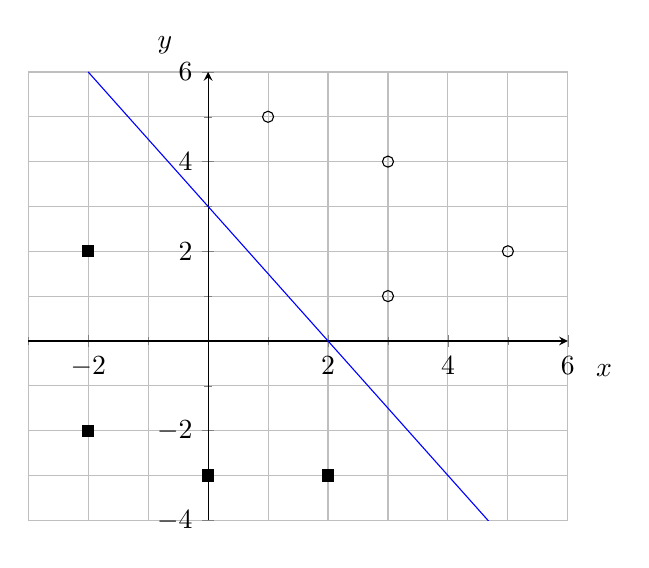
\begin{tikzpicture}
	\begin{axis}[grid=both,ymin=-4,ymax=6,xmin=-3,xmax=6,
               minor tick num=1,axis lines = middle,xlabel=$x$,ylabel=$y$,label style={at={(ticklabel cs:1.1)}},
               scatter/classes={
               	s={mark=square*,black},
               	c={mark=o}}
               ]
		% add points
		\addplot [scatter,only marks, scatter src=explicit symbolic]
			table[meta=label] {
				x   y  label
				-2 -2  s
				-2  2  s
				 0 -3  s
				 2 -3  s
				 1  5  c
				 3  1  c
				 3  4  c
				 5  2  c
			};
		% add line
		\addplot [mark=none,blue] coordinates { (-2,6) (0,3) (2,0) (6,-6) };
  \end{axis}
\end{tikzpicture}
\end{figure} \FigureHSpace
Our goal is to find a line $0=l=w_1x_1+w_2x_2-\theta$, which is equivalent to $x_2=-\frac{w_1}{w_2}x_1 + \frac{\theta}{w_1}$, that separates the circles and the squares. From the graph we see that the blue line fulfills this.\\
It's equation is given by:
\[ x_2 = -\frac{3}{2}x_1 + 3 \quad \widehat{=} \quad x_2=-\frac{w_1}{w_2}x_1 + \frac{\theta}{w_1} \]
Therefore we can choose $w_1=3$, $w_2=2$ and obtain $\theta=6$. So the network
\begin{figure}[H]
\centering
% Define block styles
\tikzstyle{plain} = [draw=none, text width=1em, text centered]
\tikzstyle{block} = [rectangle, draw, text width=2em, text centered]
\tikzstyle{arrow} = [draw, -latex']

%\resizebox{\linewidth}{!}{
	\begin{tikzpicture}[every node/.style={font=\footnotesize}, node distance=2cm, auto, >=latex']
		% Place nodes
		\node [plain] (input) {$x_1$\\$x_2$};
		\node [block, right of=input, node distance=3cm] (sum) {$\theta=6$};
		\node [plain, right of=sum] (output) {y};

		% Draw edges
		\path[->] ([yshift=0.2cm]input.east) edge node [above] {$w_1=3$} ([yshift=0.2cm]sum.west);
   	\path[->] ([yshift=-0.2cm]input.east) edge node [below] {$w_2=2$} ([yshift=-0.2cm]sum.west);
		\path[->] (sum) edge (output);
	\end{tikzpicture}
%}
\end{figure} \FigureHSpace
is able to separate our given points and can decide if another given point is in the set of squares or belongs to the set of circles.

\hspace*{-1.5em}
If we consider another set of points, displayed in the following plot:
\begin{figure}[H]
\centering
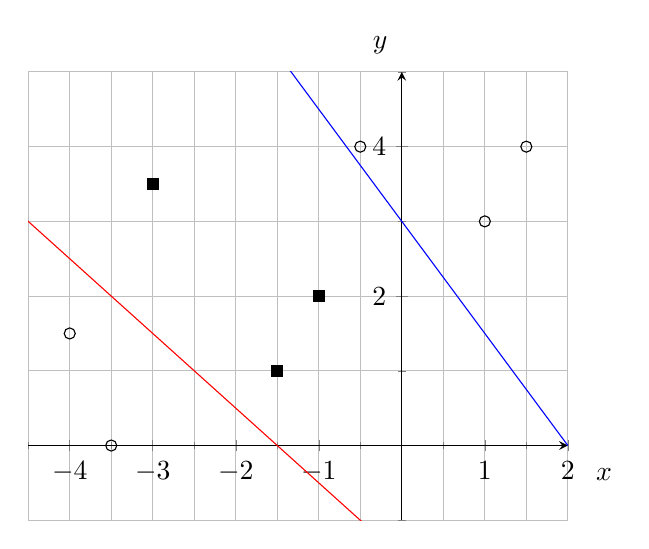
\begin{tikzpicture}
	\begin{axis}[grid=both,ymin=-1,ymax=5,xmin=-4.5,xmax=2,
               minor tick num=1,axis lines = middle,xlabel=$x$,ylabel=$y$,label style={at={(ticklabel cs:1.1)}},
               scatter/classes={
               	s={mark=square*,black},
               	c={mark=o}}
               ]
		% add points
		\addplot [scatter,only marks, scatter src=explicit symbolic]
			table[meta=label] {
				x     y   label
				-4   1.5   c
				-3.5  0    c
				-1.5  1    s
				-3   3.5   s
				-1    2    s
				-0.5  4    c
				 1    3    c
				 1.5  4    c
			};
		% add line
		\addplot [mark=none,blue] coordinates { (-2,6) (0,3) (2,0)};
		\addplot [mark=none,red]  coordinates { (-5.5,4) (-3.5,2) (-1.5,0) (0.5,-2) };
  \end{axis}
\end{tikzpicture}
\end{figure} \FigureHSpace
we see that we cannot separate them with just one line. Therefore we need at least two layers and three neurons, where the first layer neurons model the red (let's call it $l_1$) and the blue line ($l_2$). If we denote the results of the respective neurons with $y_1$ and $y_2$ we obtain the following table where $y=1$ means: \qq{The given point belongs to the set of squares}.\\
For $i=1,2$ we know: $y_i=1$ is equivalent to $l_i\geq 0$, so the point lies right of or on the line, on case of $y_i=0$ we have the point lying left of the line.
\vspace*{2mm}
\begin{center}
\begin{tabular}{|cc|c|}
\hline
\rule[-1ex]{0pt}{2.5ex} $y_1$ & $y_2$ & $y$ \\
\hline
\rule[-1ex]{0pt}{2.5ex} 0 & 0 & 0 \\
\hline
\rule[-1ex]{0pt}{2.5ex} 0 & 1 & 1 \\
\hline
\rule[-1ex]{0pt}{2.5ex} 1 & 0 & 0 \\
\hline
\rule[-1ex]{0pt}{2.5ex} 1 & 1 & 0 \\
\hline
\end{tabular}
\end{center}
\vspace*{3mm}
This table can be represented (and solved) by the following system:
\begin{figure}[H]
\centering
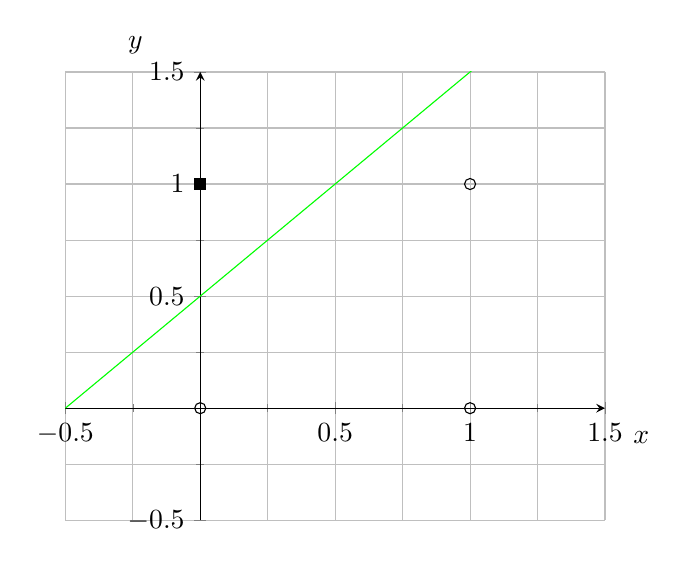
\begin{tikzpicture}
	\begin{axis}[grid=both,ymin=-0.5,ymax=1.5,xmin=-0.5,xmax=1.5,
               minor tick num=1,axis lines = middle,xlabel=$x$,ylabel=$y$,label style={at={(ticklabel cs:1.1)}},
               scatter/classes={
               	s={mark=square*,black},
               	c={mark=o}}
               ]
		% add points
		\addplot [scatter,only marks, scatter src=explicit symbolic]
			table[meta=label] {
				x     y   label
				0     0    c
				1     0    c
				1     1    c
				0     1    s
			};
		% add line
		\addplot [mark=none,green] coordinates { (-0.5,0) (1.5,2)};
  \end{axis}
\end{tikzpicture}
\end{figure} \FigureHSpace
Our next step is to calculate again the parameters for a feedforward artificial network that can divide two groups of points where the groups are given by the exemplary points above.\\
The equation for the lines are:
\begin{align*}
&l_1\, (red):  & x_2&= -x_1 - \frac{3}{2}  & & \\
 & & &\widehat{=} -\frac{w_{11}}{w_{21}}x_1 + \frac{\theta_1}{w_{21}} \\
&l_2\, (blue): & x_2&= -\frac{3}{2}x_1 + 3 \\
 & & &\widehat{=} -\frac{w_{12}}{w_{22}}x_1 + \frac{\theta_2}{w_{22}} \\
&l\, (green): & x_2&= x_1 + \frac{1}{2} \\
 & & &\widehat{=} -\frac{w_1}{w_2}x_1 + \frac{\theta}{w_2}.
\end{align*}
We obtain for example:
\begin{align*}
w_{11} &= 2, w_{21} = 2, \theta_1 = 3 \\
w_{12} &= 3, w_{22} = 2, \theta_2 = 6 \\
w_1 &= -2, w_2 = 2, \theta = 1
\end{align*}
Therefore our feedforward artificial network which separates these two groups of points is given by:
\begin{figure}[H]
\centering
% Define block styles
\tikzstyle{plain} = [draw=none, text width=1em, text centered]
\tikzstyle{block} = [rectangle, draw, text width=3em, text centered]
\tikzstyle{arrow} = [draw, -latex']

%\resizebox{\linewidth}{!}{
	\begin{tikzpicture}[every node/.style={font=\footnotesize}, node distance=1.5cm, auto, >=latex']
		% Place nodes
		\node [plain] (input1) {$x_1$};
		\node [plain, below of=input1] (spaceV) {};
		\node [plain, below of=spaceV] (input2) {$x_2$};
		\node [block, right of=input1, node distance=3cm] (sum1) {$\theta_1=3$};
		\node [block, right of=input2, node distance=3cm] (sum2) {$\theta_2=6$};
		\node [plain, right of=sum1, node distance=3cm] (spaceH) {};
		\node [block, below of=spaceH] (sum) {$\theta=1$};
		\node [plain, right of=sum] (output) {y};

		% Draw edges
		\path[->] (input1.east) edge node [above] {$w_{11}=2$} (sum1.west);
		\path[->] (input1.east) edge node [above] {$w_{12}=3$} (sum2.west);
		\path[->] (input2.east) edge node [below] {$w_{21}=2$} (sum1.west);
		\path[->] (input2.east) edge node [below] {$w_{22}=2$} (sum2.west);
		\path[->] (sum1.east) edge node [above] {$w_1=-2$} (sum.west);
		\path[->] (sum2.east) edge node [below] {$w_2=2$} (sum.west);
		\path[->] (sum) edge (output);
	\end{tikzpicture}
%}
\end{figure} \FigureHSpace
Now we presented two examples how to obtain the parameters for different separation problems.\\
In the next part we present the basic principle of obtaining the parameters with an algorithm via supervised learning.


\subsection{Supervised learning}
In artificial intelligence we speak from supervised learning if the network gets some positive and negative examples and calculates the parameters of the network via updating by itself. Afterwards the quality of the network is being tested by some exemplary test-sets.\\
For example in the part above we got some point sets where we knew that the circles were \qq{negative} examples and the squares \qq{positive} examples.

\subsubsection*{Update}
In the case of an $n$-input, one-output neuron we can adapt the following learning rule:\\
Beginning from default (e.g. 0) or other specified starting values we adjust the respective weights $w_j,\,j=1,\hdots,n$ and $\theta$ with an update $\Delta w_j,\,j=1,\hdots,n$ and $\Delta \theta$.\\
Let $j\in\{1,\hdots,n\}$ and $s\in\N$ be the number of the sample we are processing. Our starting values are subscribed with $w_j(0)$ and $\theta(0)$.\\
The learning rule is calcutated as following:
\begin{align*}
w_j(s+1) &= w_j(s) + \Delta w_j(s), & \theta(s+1) &= \theta(s) + \Delta \theta(s), \\
\Delta w_j(s) &= x_j\delta(s), & \Delta \theta(s) &= \delta(s), \\
\delta(s) &= t-y(s),
\end{align*}
where $t$ is the output of the given sample and $y(s)$ the computed output for the sample. We know that $\delta(s)\in\{-1,0,1\}$ because $t,y(s)\in\{0,1\}$. Therefore we obtain for the updates
\[ \Delta w_j(s)=\begin{cases}
	x_j, &\delta(s)=1 \\
	0, &\delta(s)=0 \\
	-x_j, &\delta(s)=-1
\end{cases}\quad \text{ and }\quad \Delta \theta(s)=\begin{cases}
	1, &\delta(s)=1 \\
	0, &\delta(s)=0 \\
	-1, &\delta(s)=-1
\end{cases} \]
Another approach for not linearly separable sets is the gradient of the steepest descend. Herefore we mostly have a smooth activation function $F$ and calculate the least mean squared error, which we use with a specified learning rate in the update rule.\\
We didn't treat this approach in this lecture.


%%%%% Content - END %%%%%
